\documentclass[default]{beamer}
\setbeamertemplate{navigation symbols}{}

\usetheme{CambridgeUS}
\useoutertheme{infolines}
%\usecolortheme{crane}

\usepackage{cmap}							% Поддержка поиска русских слов в PDF (pdflatex)
\usepackage[T2A]{fontenc}       			%поддержка кириллицы
\usepackage[utf8]{inputenc}					% Выбор языка и кодировки
\usepackage[english, russian]{babel}

\graphicspath{{../../images/mpf/}} 			% Пути к изображениям

\makeatletter
\setbeamertemplate{footline}
{
	\leavevmode%
	\hbox{%
		\begin{beamercolorbox}[wd=.333333\paperwidth,ht=2.25ex,dp=1ex,center]{author
				in head/foot}%
			\usebeamerfont{author in
				head/foot}\insertshortauthor~~\beamer@ifempty{\insertshortinstitute}{}{(\insertshortinstitute)}
		\end{beamercolorbox}%
		\begin{beamercolorbox}[wd=.333333\paperwidth,ht=2.25ex,dp=1ex,center]{title in
				head/foot}%
			\usebeamerfont{title in head/foot}\insertshorttitle
		\end{beamercolorbox}%
		\begin{beamercolorbox}[wd=.333333\paperwidth,ht=2.25ex,dp=1ex,right]{date in
				head/foot}%
			\usebeamerfont{date in head/foot}\insertshortdate{}\hspace*{2em}
			\insertframenumber{}\hspace*{2ex} 
		\end{beamercolorbox}
	}%
	\vskip0pt%
}

\setbeamertemplate{bibliography entry title}{}
\setbeamertemplate{bibliography entry location}{}
\setbeamertemplate{bibliography entry year}{}
\setbeamertemplate{bibliography entry note}{}
\bibliographystyle{gost2008p}

\begin{document}
	
	\title[ART Гроссберга]{Теория адаптивного резонанса Гроссберга}
	\author[Панов]{Александр Панов}
	\institute[ИСА РАН]{ИСА РАН}
	\date{13 февраля 2015~г.} 
	
	\begin{frame}
		\titlepage
	\end{frame}
	
	\begin{frame}
		\frametitle{Гроссберг}
		
		\begin{itemize}
			\item Стефан Гроссберг, 75 лет "--- специалист по когнитивным наукам, нейрофизиолог,~математик.
			\item Профессор Бостонского университета.
			\item Scopus: более 380 статей, h-индекс "--- 64.
			\item Работы с количеством цитирований более 1000:

			{
				\scriptsize
				\nocite{*}
				\inputencoding{cp1251}
				\bibliography{../../biblio/ikm}
				\inputencoding{utf8}
			}
		\end{itemize}
	\end{frame}
	
	\begin{frame}
		\frametitle{Основные проблемы}
		
		\begin{itemize}
			\item Проблема соотношения стабильности и пластичности в восприятии.
			\item Принцип дополняющих когнитивных процессов.
			\item Принцип послойной организации всех когнитивных процессов.
			\item Все состояния сознания являются состояниями резонанса.
		\end{itemize}
		
		\begin{figure}
			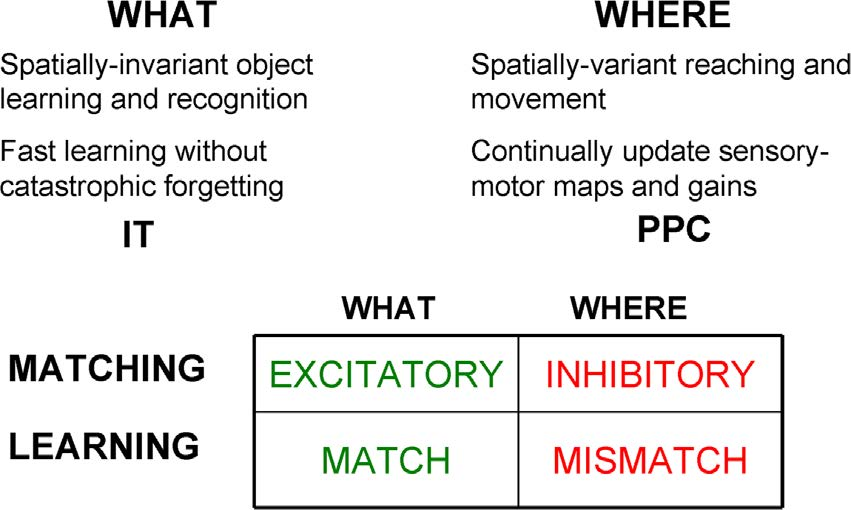
\includegraphics[width=0.5\textwidth]{grossberg_compl}
		\end{figure}
		
	\end{frame}	

	\begin{frame}
		\frametitle{Что, где и как в коре головного мозга}
		
		\begin{columns}
			\begin{column}{0.6\textwidth}
				\footnotesize
				Дорсальный (Что?) и вентральный (Где?, Как?) пути обработки информации.
				\begin{itemize}
					\item Retina/LGN "--- сетчатка/боковое коленчатое ядро.
					\item V1, V2, V3, V4 "--- первичная и вторичные зоны зрительной коры.
					\item IT "--- нижневисочная (инферотемпоральная) зона коры.
					\item ORB "--- глазнично"--~лобная (орбитофронтальная) зона коры.
					\item LIP "--- латеральная межтеменная (интрапариетальная) зона коры.
					\item PPC "--- задняя теменная (париетальная) зона коры.
					\item PFC "--- передняя лобная зона коры.
					\item FEF "--- глазодвигательная кора.
				\end{itemize}
			\end{column}
			\begin{column}{0.4\textwidth}
				\vspace*{-5mm}
				\begin{figure}
					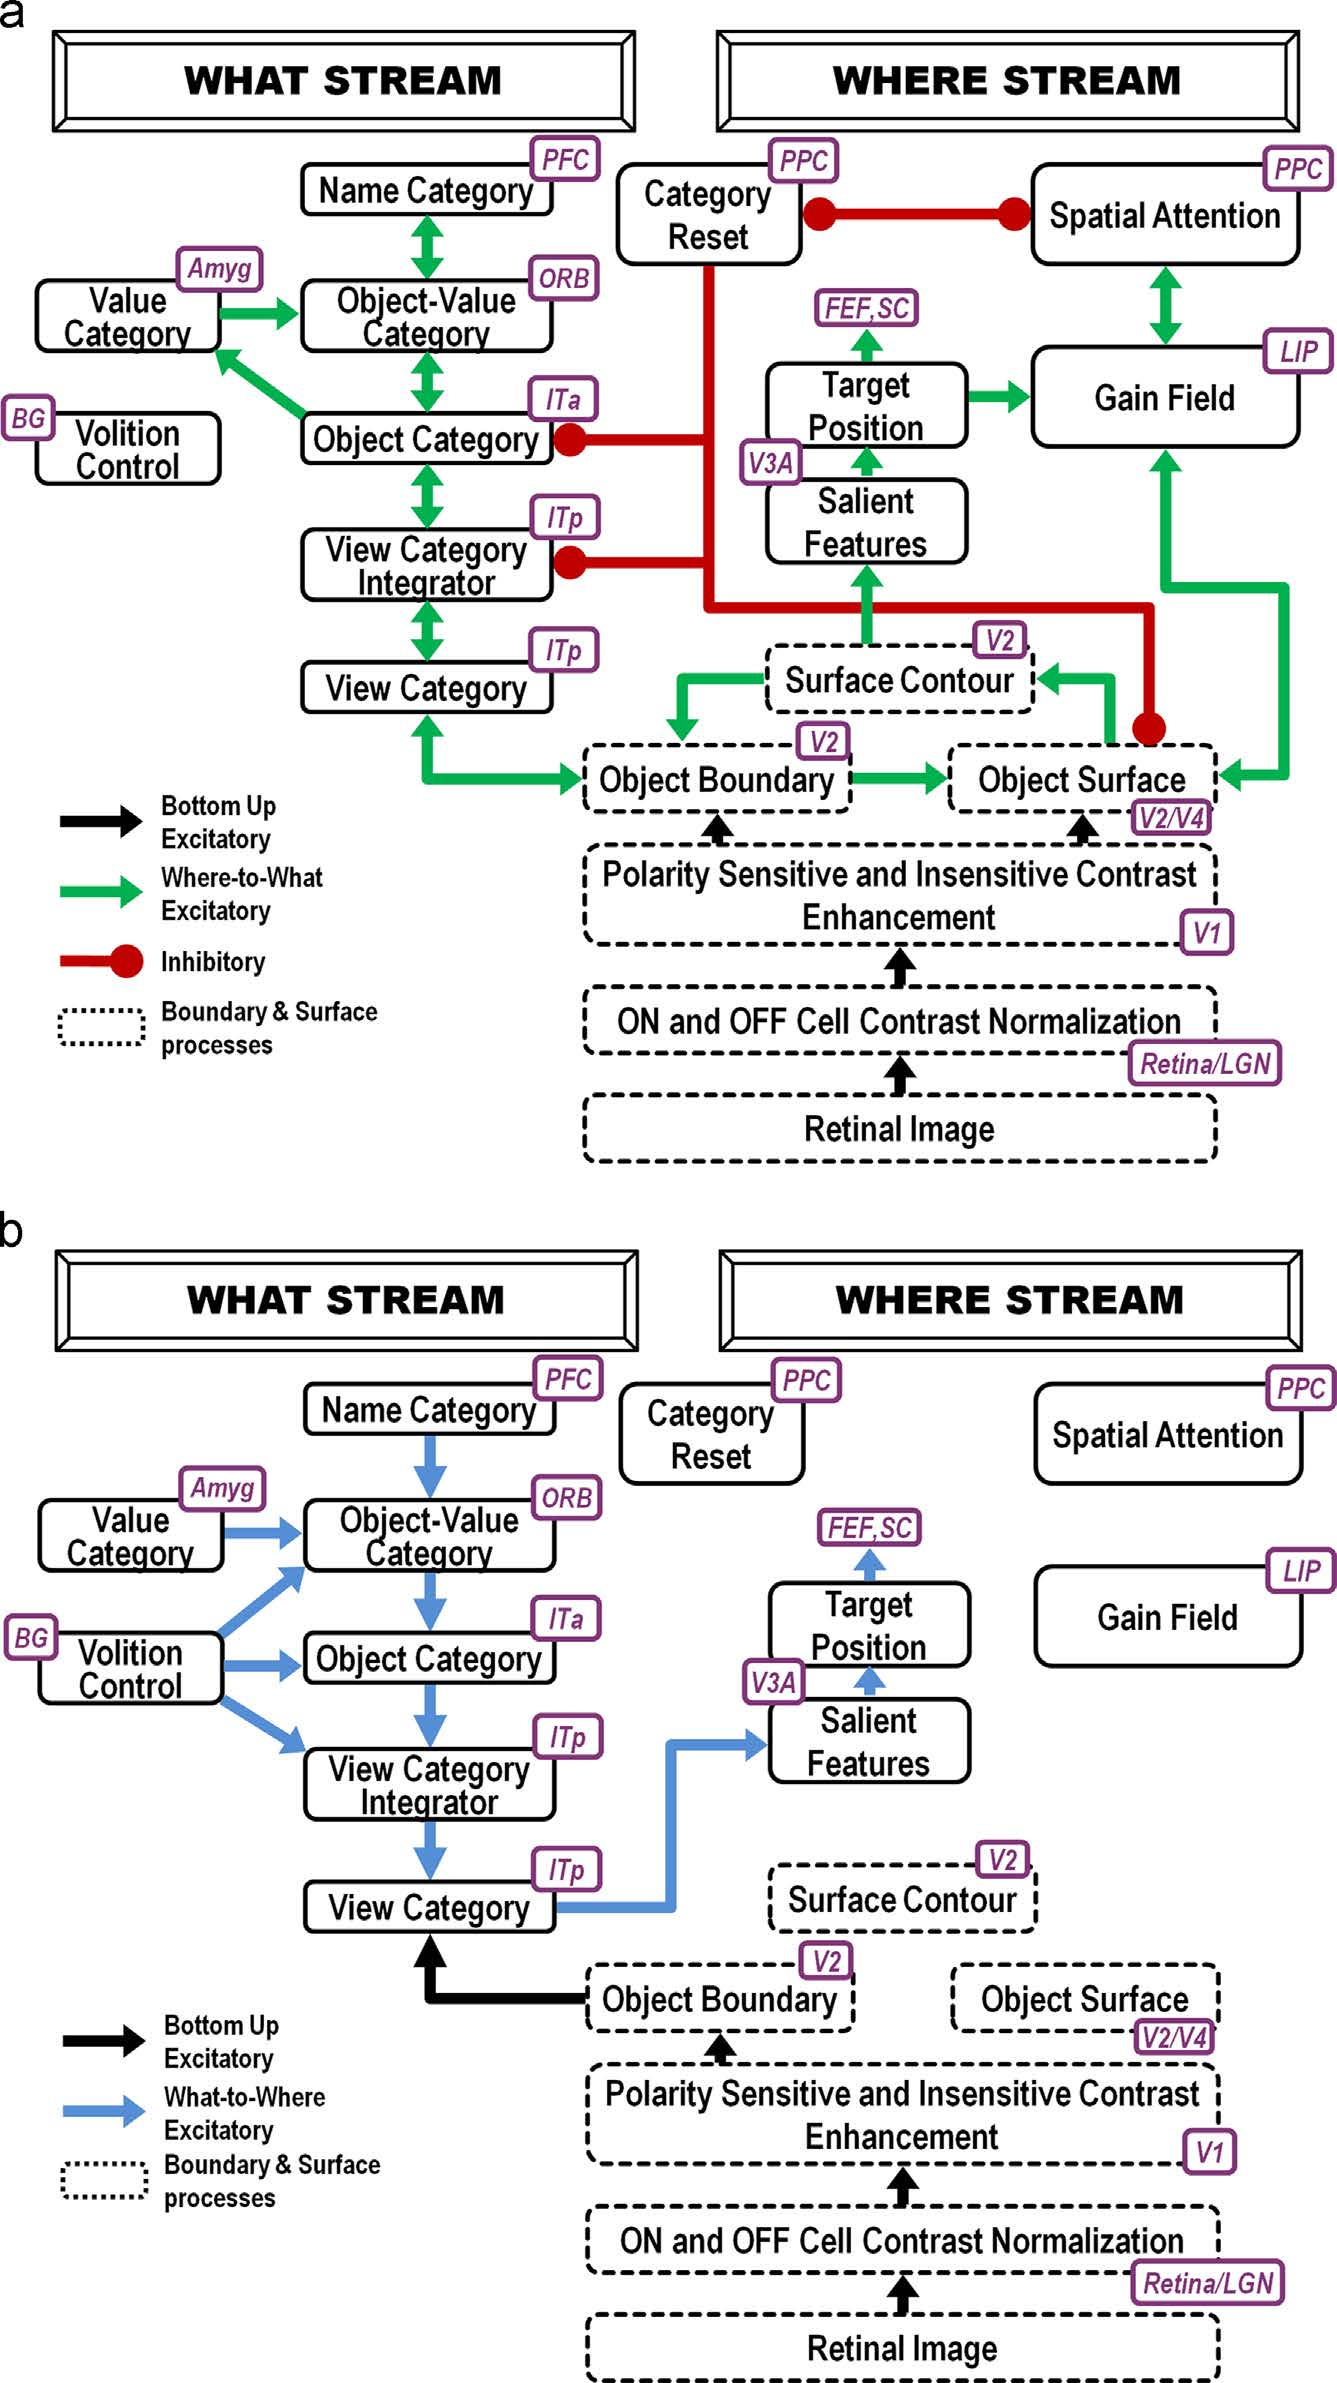
\includegraphics[width=0.9\textwidth]{grossberg_streams}
				\end{figure}
				
			\end{column}
		\end{columns}
	\end{frame}

	\begin{frame}
		\frametitle{Нейронная сеть ART-1}
		\onslide<1->{
			\begin{figure}
				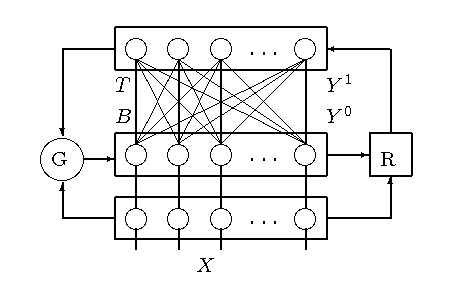
\includegraphics[width=0.35\textwidth]{art_1}
			\end{figure}
		}
		\begin{overlayarea}{\textwidth}{.5\textheight}
			\only<1>{
				\begin{itemize}
					\item Четыре функциональных модуля: слой сравнения, слой распознавания и два управляющих нейрона: сброса $R$ и управления $G$.
					\item Вектора $X, Y^0, Y^1$ "--- двоичные вектора.
					\item Для нейронов слоя сравнения используется правило $2/3$.
				\end{itemize}
			}
			\only<2>{
				\footnotesize
				\begin{itemize}
					\item \textbf{Начальная фаза}: $G=0$ при $X=\{0,\dots,0\}$; при поступлении ненулевого $X$ принимаем $G=1$, $Y^0=X$ и определяем $Y^1=\{y_1^1,\dots,y_n^1\}$, $\forall i\not =w\ y_i^1=0, y_w^1=1$, где $w$ "--- индекс нейрона-победителя ($\max_j\sum_i y_i^0*b_{ij}$) в слое распознавания, обнуляем управление $G=0$.
					\item \textbf{Фаза сравнения}: Новый выход слоя сравнения $Y^0=\{t_{1w},\dots,t_{mw}\}\wedge X$; если $\|Y^0\|/\|X\|>\rho$, то завершаем процесс, иначе возникает сигнал сброса, подавляется нейрон-победитель и начинается фаза поиска.
					\item \textbf{Фаза поиска}: так как нейрон победитель подавлен, то $R$ обнуляется, $G=0$, $Y^0=X$, определяется новый нейрон-победитель и снова переходим к фазе сравнения.
				\end{itemize}
			}
			\only<3>{
				\footnotesize
				Окончание итерационного процесса:
				\begin{itemize}
					\item Найдётся запомненная категория, сходство которой с входным вектором X будет достаточным для успешной классификации. После этого запускается \textbf{фаза обучения}, в котором модифицируются веса $b_{iw}$ и $t_{iw}$ матриц $B$ и $T$ для победившего нейрона.
					\item В процессе поиска все запомненные категории окажутся проверенными, но ни одна из них не дала требуемого сходства. В этом случае входной образ $X$ объявляется новым для нейросети, и ему выделяется новый нейрон в слое распознавания.
				\end{itemize}
			}	
		\end{overlayarea}
	
	\end{frame}

	\begin{frame}
		\frametitle{Фаза обучения}
		
		\begin{itemize}
			\item Начальный значения матриц $B$ и $T$ должны удовлетворять соотношениям: $b_{ij}<L/(L-1+m)$, $t_{ij}=1$, $m$ "--- размерность входных данных (вектора $X$).
			\item При нахождении подходящей категории по вектору $Y^0=\{y_1^0,\dots,y_m^0\}$ $b_{ij}=(L*y_i^0)/(L-1+\sum_k y_k^0)$, $\forall i\ t_{ij}=y_i^0$.
			\item Обучение, таким образом, сопровождается занулением все большего числа компонент матрицы $T$, оставшиеся ненулевыми компоненты определяют множество критических черт найденных категории.
		\end{itemize}
		\begin{figure}
			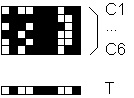
\includegraphics[width=0.3\textwidth]{art_learn}
		\end{figure}
	\end{frame}

	\begin{frame}
		\frametitle{Принцип многослойности}
		
		\begin{figure}
			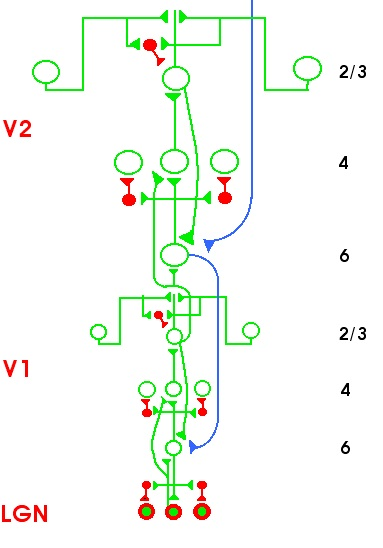
\includegraphics[width=0.45\textwidth]{art_neuro}
		\end{figure}
	\end{frame}
			
	\begin{frame}
		\frametitle{Дальнейшее развитие}
		
		\begin{itemize}
			\item ART-2 "--- переход от двоичных значений к непрерывным (действительным).
			\item ART-3 "--- добавление нескольких слоёв для сжатия информации и абстрагирования. Резонанс возникает на некотором уровне иерархии. Введён механизм рефрактерного торможения.
			\item FuzzyART "--- введение элементов нечёткой логики.
			\item ARTMAP, pART "--- комбинация двух блоков ART-1 и ART-2 для регулировки параметра сброса (бдительности).
			\item Много прикладных моделей: dARTEX,
		\end{itemize}
	\end{frame}
	%	\begin{frame}
	%		\frametitle{Цели курса}
	%		
	%		\begin{itemize}
	%			\item
	%		\end{itemize}
	%	\end{frame}
	
\end{document}
	
	
